\chapter{Mask Catalogue}
\label{app:masks}

This appendix gives the precise specification of the five mask
families used in Chapter~\ref{ch:architecture}. The shorthand
$(T, h_{p}, w_{p}) = (14, 16, 16)$ refers to the number of frames
and the patch grid that the encoder sees per window.

\section{Definitions}
\label{app:masks-defs}

Let $r \in [0, 1]$ be the per-window mask ratio. The five
families are sampled independently per window from the policy
distribution of Section~\ref{sec:arch-mask}.

\begin{description}
\item[Short tube.] A rectangular patch in the $(h_{p}, w_{p})$
grid is selected at random and masked across all $T$ frames. The
spatial area is set such that the time-averaged mask ratio matches
$r/n$ for $n = 2$ tube events per window. Implemented in
\texttt{mask\_catalog.\_sample\_tube\_one} with
$\mathtt{area} = 0.15$.

\item[Long tube.] Same as short tube with
$\mathtt{area} = 0.40$. Used in tube-heavy mixtures.

\item[Future block.] All tokens at frames
$t \geq t_{\text{in}}$ are masked; tokens at $t < t_{\text{in}}$
are left visible. Implemented in
\texttt{mask\_catalog.\_sample\_future\_one}; the masked fraction
is $\mathtt{frac} = (t_{\text{out}}) / T$.

\item[Cross-time.] A random subset of the $T$ frames is selected
and masked across the entire spatial grid; the complementary
subset is left fully visible. Implemented in
\texttt{mask\_catalog.\_sample\_cross\_time\_one} with
$\mathtt{frac} = 0.30$.

\item[Tail.] The last $t_{\text{out}}$ frames are masked across
the entire spatial grid (a deployment-style mask used to warm up
the curriculum). Implemented in
\texttt{mask\_catalog.\_sample\_tail\_one}.
\end{description}

\section{Curriculum}
\label{app:masks-curr}

The two-stage slow curriculum used throughout
Chapter~\ref{ch:experiments} is parameterised by
$\mathit{tail\_only\_pct}$ and $\mathit{warmup\_pct}$.
For an $N$-epoch run, epochs
$[0, \mathit{tail\_only\_pct} \cdot N)$ use only the tail family;
epochs
$[\mathit{tail\_only\_pct} \cdot N, \mathit{warmup\_pct} \cdot N)$
interpolate linearly between tail and the full mixture; and
epochs $[\mathit{warmup\_pct} \cdot N, N]$ use the full mixture.
The slow setting is $(0.25, 0.40)$; the abandoned fast setting
was $(0.10, 0.20)$ and is recorded as Finding~F7.

\section{One realisation per family}
\label{app:masks-fig}

\begin{figure}[htbp]
\centering
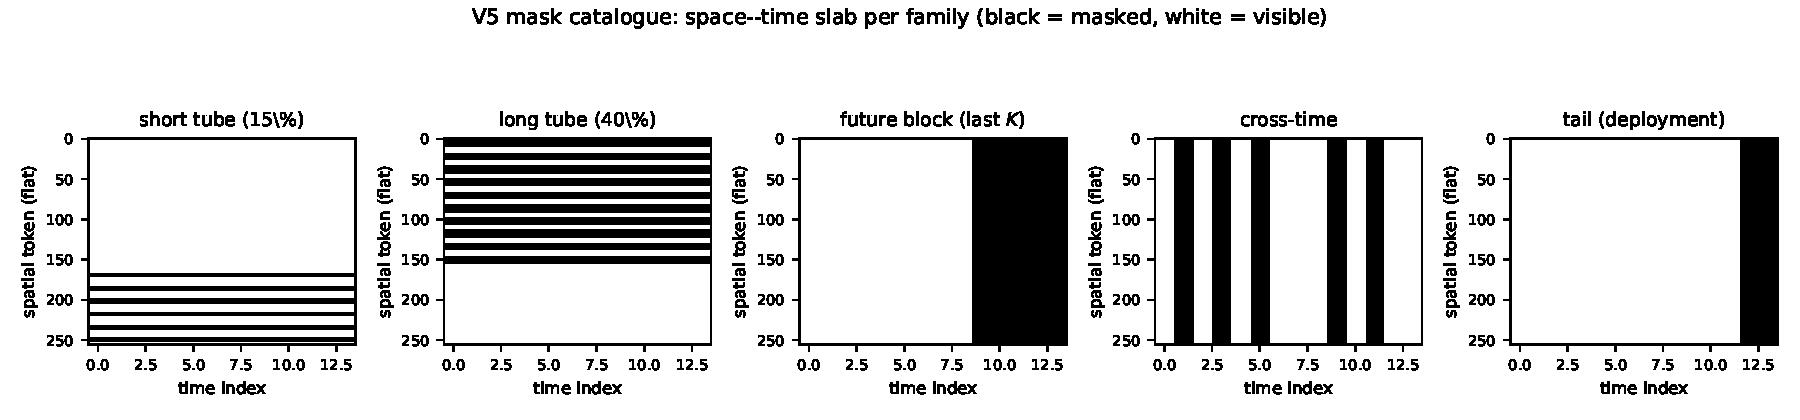
\includegraphics[width=0.95\linewidth]{assets/figures/mask_catalog.pdf}
\caption{One realisation of each mask family at
$(T, h_{p}, w_{p}) = (14, 16, 16)$, rendered from
\texttt{solarflare\_data.mask\_catalog}. White denotes masked
tokens; black denotes visible tokens. The displayed frame is the
first frame for short/long tubes, the final frame for the future
block and the tail family, and a frame chosen from the masked
subset for cross-time.}
\label{fig:masks}
\end{figure}
